% Compile from this directory with Tectonic.
\documentclass[aspectratio=169,11pt]{beamer}
\usepackage[T1]{fontenc}
\usepackage{lmodern}
\usepackage{graphicx}
\usepackage{amsmath,amssymb}
\usepackage{booktabs}
\usepackage{tikz}
\usetikzlibrary{arrows.meta,positioning,calc}

\definecolor{ink}{HTML}{14283F}
\definecolor{teal}{HTML}{087F8C}
\definecolor{muted}{HTML}{52677B}
\definecolor{light}{HTML}{E8F2F2}
\definecolor{accent}{HTML}{C96B37}
\definecolor{wall}{HTML}{253447}
\setbeamercolor{normal text}{fg=ink,bg=white}
\setbeamercolor{frametitle}{fg=ink,bg=white}
\setbeamercolor{title}{fg=ink}
\setbeamercolor{structure}{fg=teal}
\setbeamerfont{frametitle}{series=\bfseries,size=\Large}
\setbeamerfont{title}{series=\bfseries,size=\huge}
\setbeamerfont{subtitle}{size=\large}
\setbeamertemplate{navigation symbols}{}
\setbeamertemplate{itemize item}{\raisebox{0.15ex}{\scriptsize$\blacktriangleright$}}
\setbeamertemplate{footline}{%
  \hfill\scriptsize\color{muted}\insertframenumber/\inserttotalframenumber
  \hspace{0.6cm}\vspace{0.25cm}}
\setbeamertemplate{frametitle}{%
  \vspace{0.25cm}\insertframetitle\par\vspace{0.08cm}
  {\color{teal}\rule{\textwidth}{0.9pt}}}
\tikzset{
  flow/.style={draw=teal,very thick,rounded corners=2pt,align=center,
    minimum height=0.84cm,fill=white,inner sep=5pt},
  soft/.style={draw=muted,rounded corners=2pt,align=center,
    minimum height=0.8cm,fill=light,inner sep=5pt},
  arr/.style={-{Latex[length=2.3mm]},thick,draw=ink}
}
\graphicspath{{assets/}}

\title{Generalization in Reinforcement Learning}
\subtitle{ActorDQN vs DQN}
\author{Xiaojie Gu}
\institute{University of Wuerzburg}
\date{}

\begin{document}

% 1 — title
\begin{frame}[plain]
  \vspace{1.25cm}
  {\color{teal}\rule{1.5cm}{3pt}}\par\vspace{0.6cm}
  {\usebeamerfont{title}\color{ink}\inserttitle\par}
  \vspace{0.28cm}
  {\usebeamerfont{subtitle}\color{muted}\insertsubtitle\par}
  \vfill
  {\large\insertauthor}\par\vspace{0.08cm}
  {\color{muted}\insertinstitute}\par\vspace{0.12cm}
  {\small\color{muted}First Advisor: Mr. Sebastian Griesbach
    \quad|\quad Supervisor: Prof. Dr. Carlo D\textquoteright{}Eramo}\par
  \vspace{0.8cm}
  \hfill{\scriptsize\color{muted}This presentation was made with assistance from GPT-6 Sol under the guidance of my hand draft.}\par
  \vspace{0.15cm}
\end{frame}

% 2 — outline
\begin{frame}{Outline}
  \vspace{0.25cm}
  \begin{enumerate}\setlength{\itemsep}{0.44cm}
    \item Introduction
    \item Environment design
    \item Model design: DQN and ActorDQN
    \item Experimental results
  \end{enumerate}
\end{frame}

% 3 — robotics generalization
\begingroup
\colorlet{teal}{black}
\colorlet{accent}{black}
\begin{frame}{Introduction: generalization in robotics}
  \begin{columns}[T,onlytextwidth]
    \begin{column}{0.49\textwidth}
      {\color{teal}\bfseries Training condition}\par\vspace{0.10cm}
      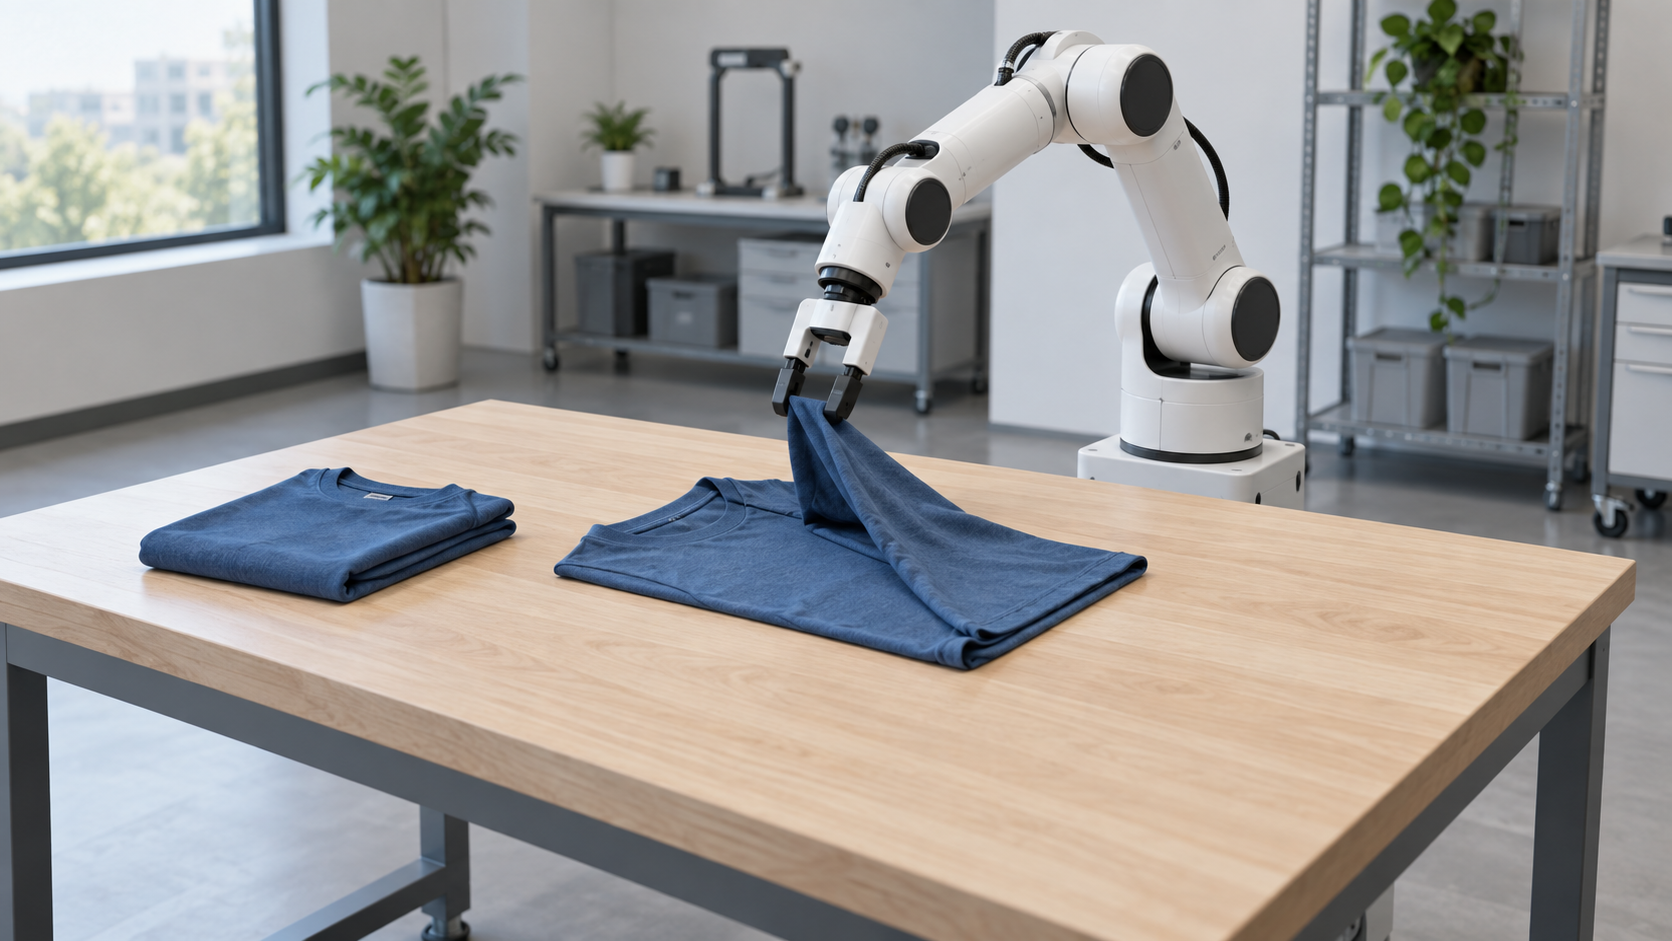
\includegraphics[width=\linewidth]{robot-train.png}
      \par\vspace{0.12cm}
      \small Table height: 1.0 m \quad Garment: T-shirt\par
      \small\color{teal}Neat fold in a familiar setting
    \end{column}
    \begin{column}{0.49\textwidth}
      {\color{accent}\bfseries Unseen test condition}\par\vspace{0.10cm}
      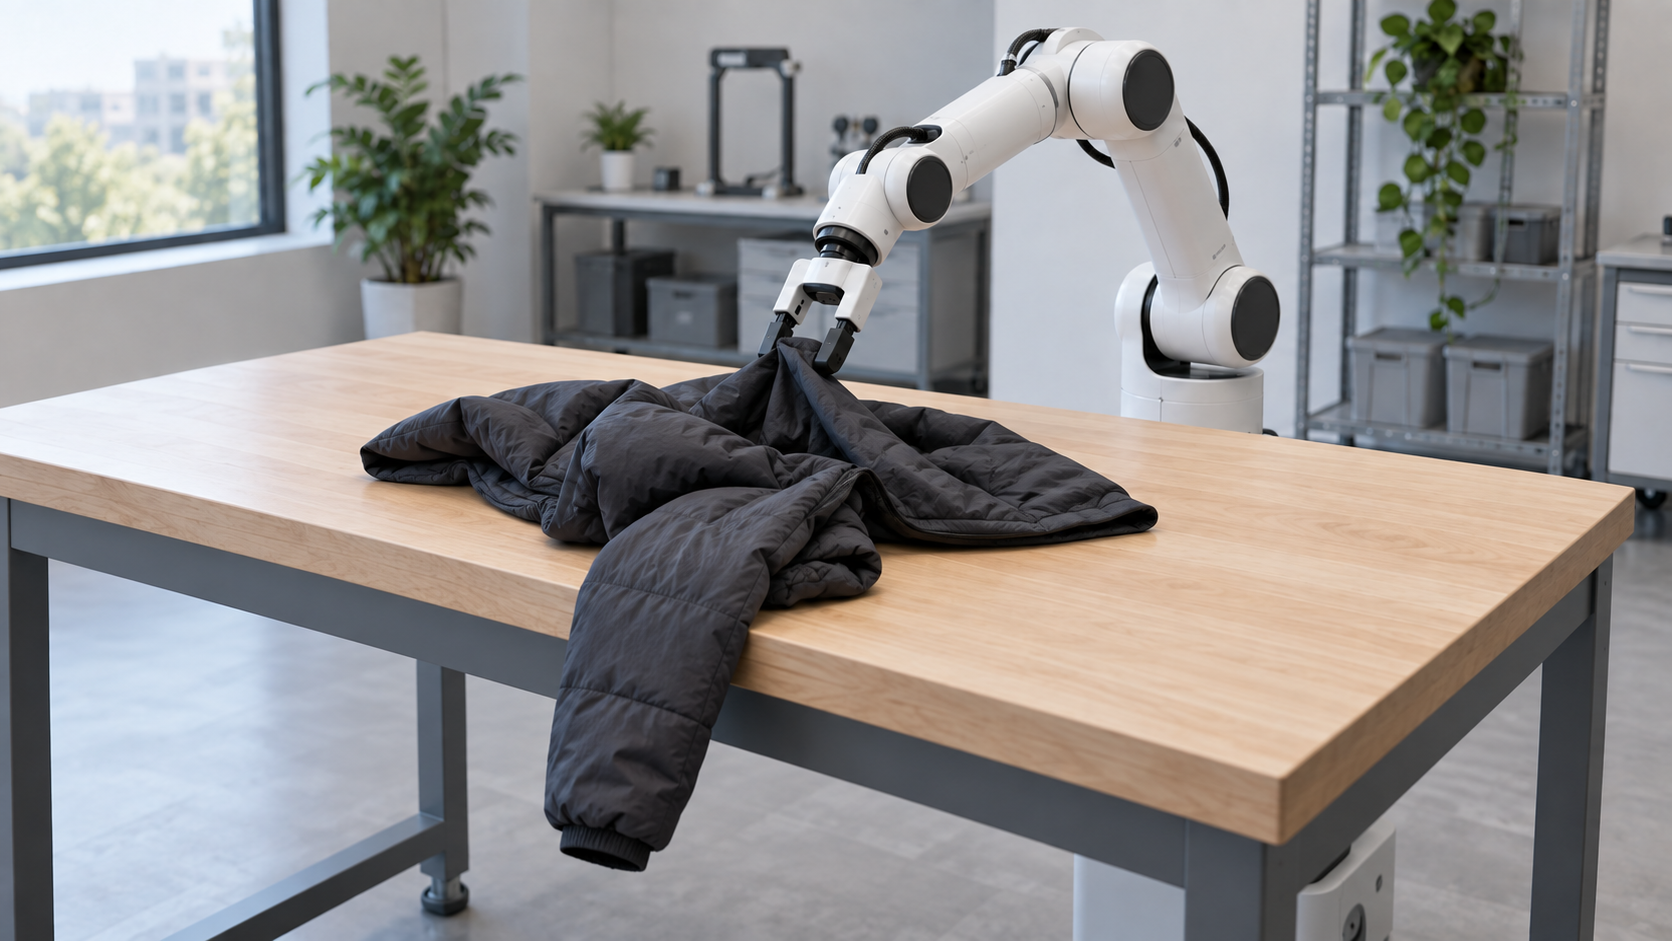
\includegraphics[width=\linewidth]{robot-test.png}
      \par\vspace{0.12cm}
      \small Table height: 1.2 m \quad Garment: jacket\par
      \small\color{accent}Unsuccessful fold after the change
    \end{column}
  \end{columns}
  \vspace{0.30cm}
  \small\color{muted}Success in training does not guarantee success when conditions change.
\end{frame}
\endgroup

% 4 — video
\begin{frame}{Generalization in robotics: Unitree video}
  \begin{columns}[c,onlytextwidth]
    \begin{column}{0.38\textwidth}
      \centering
      \href{run:../unitree/1787627734150609_english_male.mp4}{%
        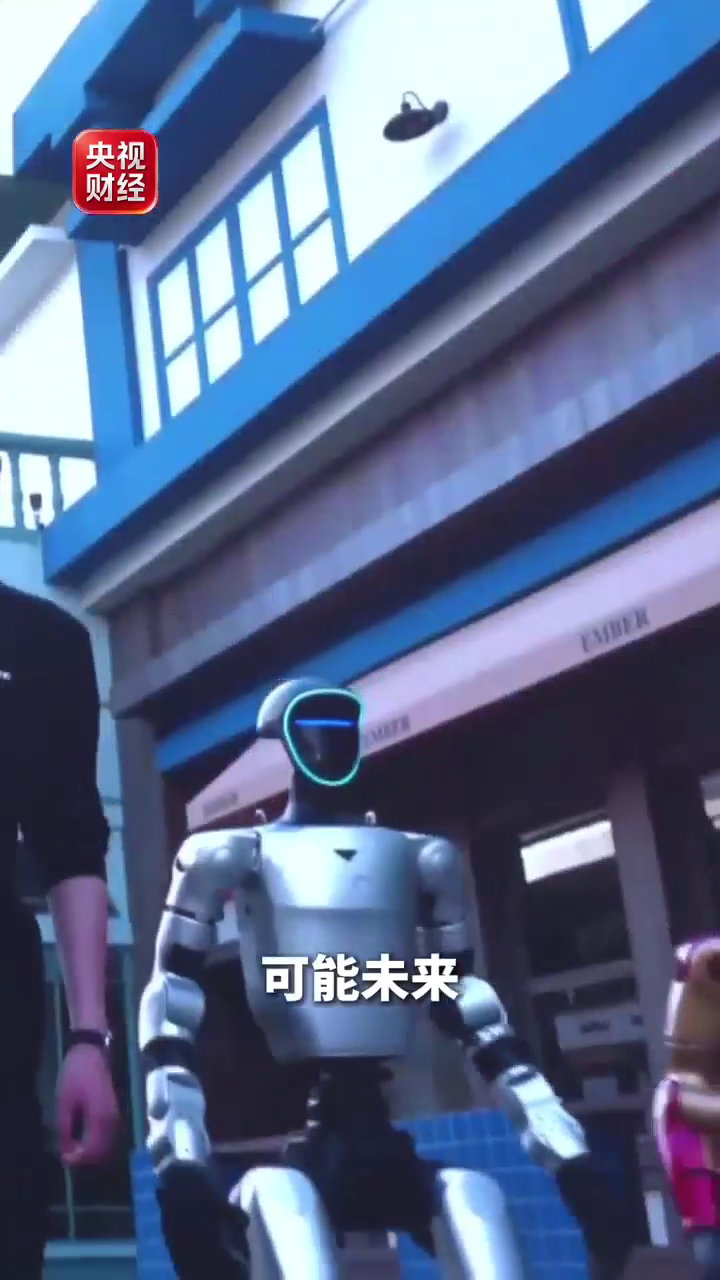
\includegraphics[height=5.0cm,keepaspectratio]{unitree-poster.png}}
    \end{column}
    \begin{column}{0.58\textwidth}
      \Large A real-world robotics example\par\vspace{0.42cm}
      \normalsize
      \href{run:../unitree/1787627734150609_english_male.mp4}{}
      \par\vspace{0.35cm}
      \small\color{muted}
    \end{column}
  \end{columns}
\end{frame}

% 5 — environment outline
\begin{frame}{Environment Design}
  \vspace{0.35cm}
  \begin{enumerate}\setlength{\itemsep}{0.70cm}
    \item \textbf{Regulation}\par
    \item \textbf{Procedural maze}\par
  \end{enumerate}
\end{frame}

% 6 — regulation
\begin{frame}{Regulation: no shared optimal solution}
  \centering
  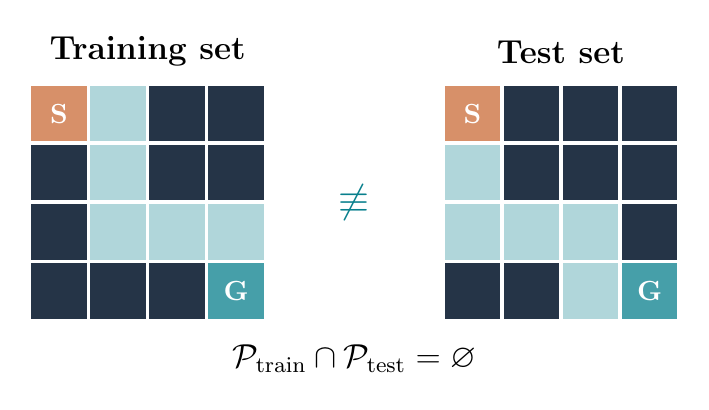
\begin{tikzpicture}[x=0.75cm,y=0.75cm]
    \node[font=\large\bfseries] at (2,4.55) {Training set};
    \node[font=\large\bfseries] at (9,4.55) {Test set};
    \fill[wall] (0,0) rectangle (4,4);
    \fill[wall] (7,0) rectangle (11,4);
    \foreach \x/\y in {0/3,1/3,1/2,1/1,2/1,3/1,3/0}
      \fill[teal!32] (\x,\y) rectangle ++(1,1);
    \foreach \x/\y in {7/3,7/2,7/1,8/1,9/1,9/0,10/0}
      \fill[teal!32] (\x,\y) rectangle ++(1,1);
    \fill[accent!75] (0,3) rectangle ++(1,1);
    \fill[accent!75] (7,3) rectangle ++(1,1);
    \fill[teal!75] (3,0) rectangle ++(1,1);
    \fill[teal!75] (10,0) rectangle ++(1,1);
    \draw[step=1,white,line width=1.3pt] (0,0) grid (4,4);
    \draw[step=1,white,line width=1.3pt] (7,0) grid (11,4);
    \node[font=\bfseries,text=white] at (0.5,3.5) {S};
    \node[font=\bfseries,text=white] at (7.5,3.5) {S};
    \node[font=\bfseries,text=white] at (3.5,0.5) {G};
    \node[font=\bfseries,text=white] at (10.5,0.5) {G};
    \node[font=\Large,text=teal] at (5.5,2) {$\not\equiv$};
    \node[font=\large] at (5.5,-0.65)
      {$\mathcal P_{\rm train}\cap\mathcal P_{\rm test}=\varnothing$};
  \end{tikzpicture}
  \par\vspace{0.12cm}
  \small\color{muted}Each original maze and its variations stay in one split; the intended shortest path does not cross splits.
\end{frame}

% 7 — procedural maze figures
\begin{frame}{Procedural Maze}
  \begin{columns}[T,onlytextwidth]
    \begin{column}{0.48\textwidth}
      \textbf{1. Enumerate start--goal pairs}\par\vspace{0.15cm}
      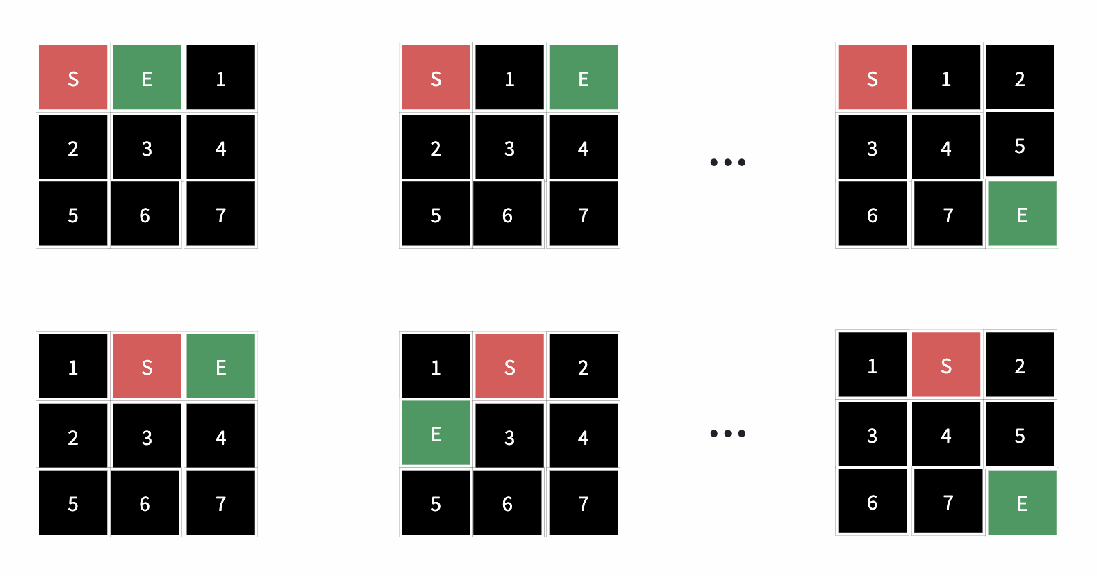
\includegraphics[width=\linewidth]{report-figure2.png}
    \end{column}
    \begin{column}{0.50\textwidth}
      \textbf{2. Generate valid paths}\par\vspace{0.15cm}
      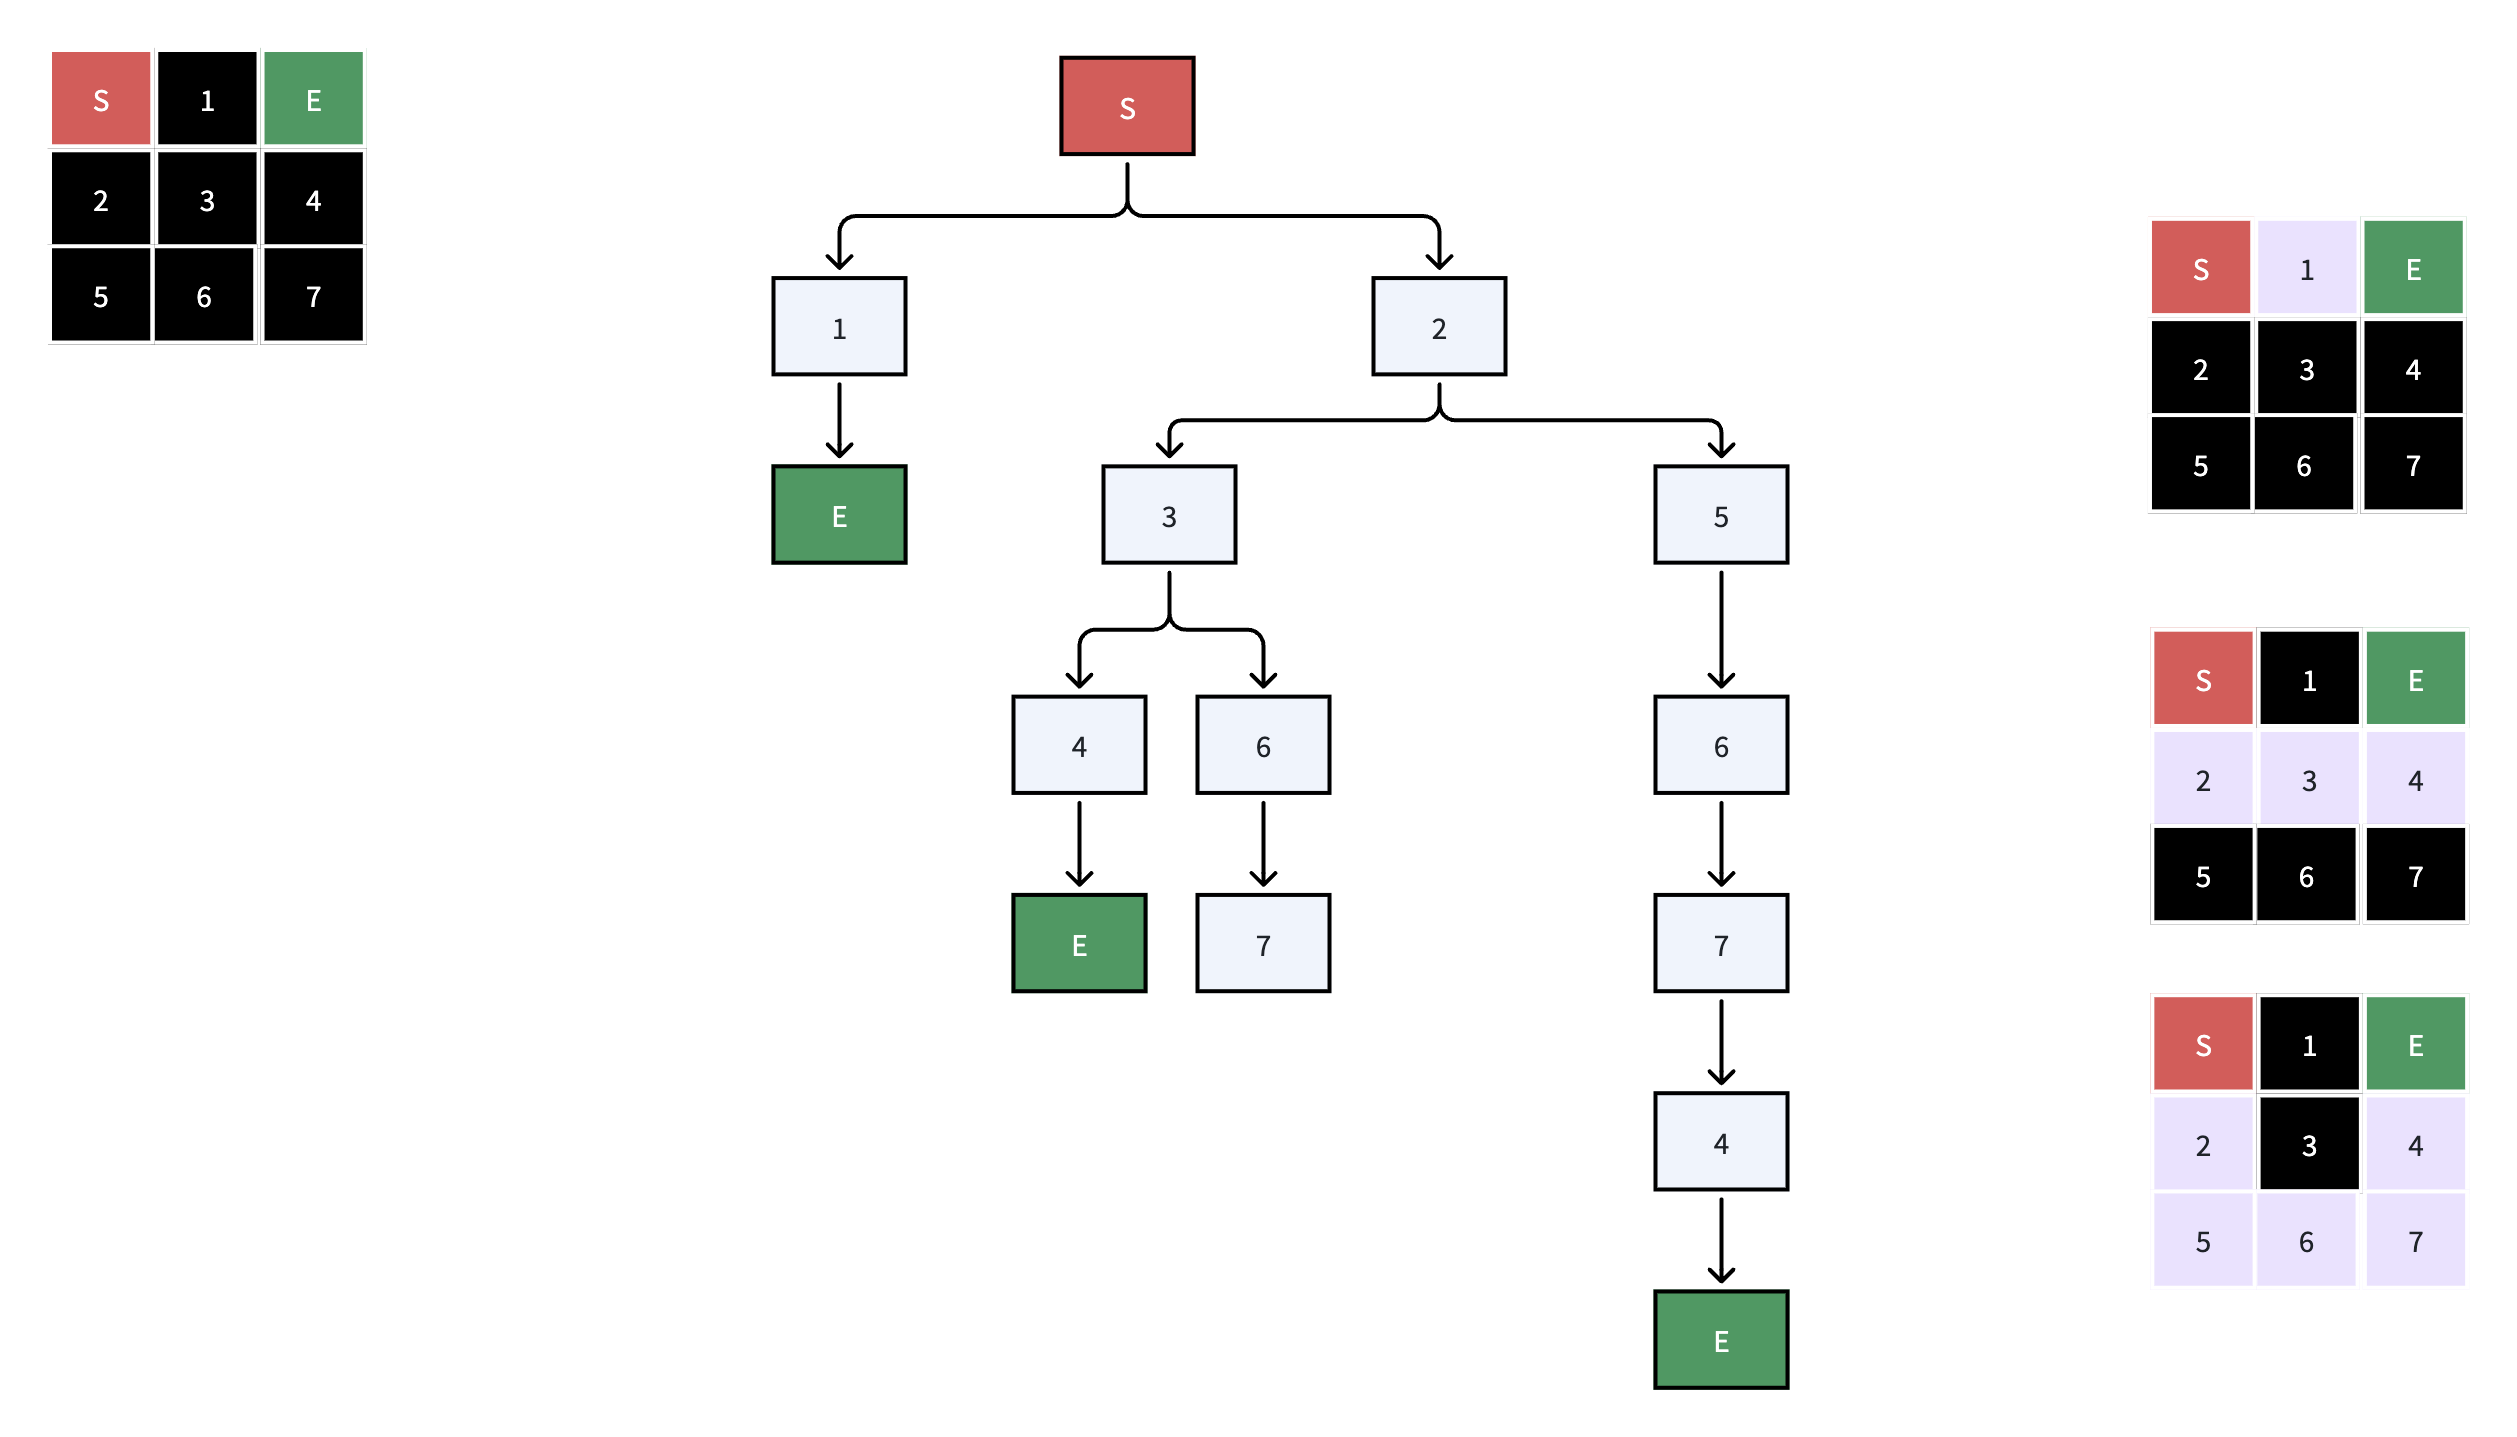
\includegraphics[width=\linewidth]{report-figure3.png}
    \end{column}
  \end{columns}
\end{frame}

% 8 — model outline
\begin{frame}{Model Design}
  \vspace{0.35cm}
  \begin{enumerate}\setlength{\itemsep}{0.70cm}
    \item \textbf{DQN}\par
    \item \textbf{ActorDQN}\par
  \end{enumerate}
\end{frame}

% 9 — DQN architecture
\begin{frame}{Model Design: DQN}
  \centering
  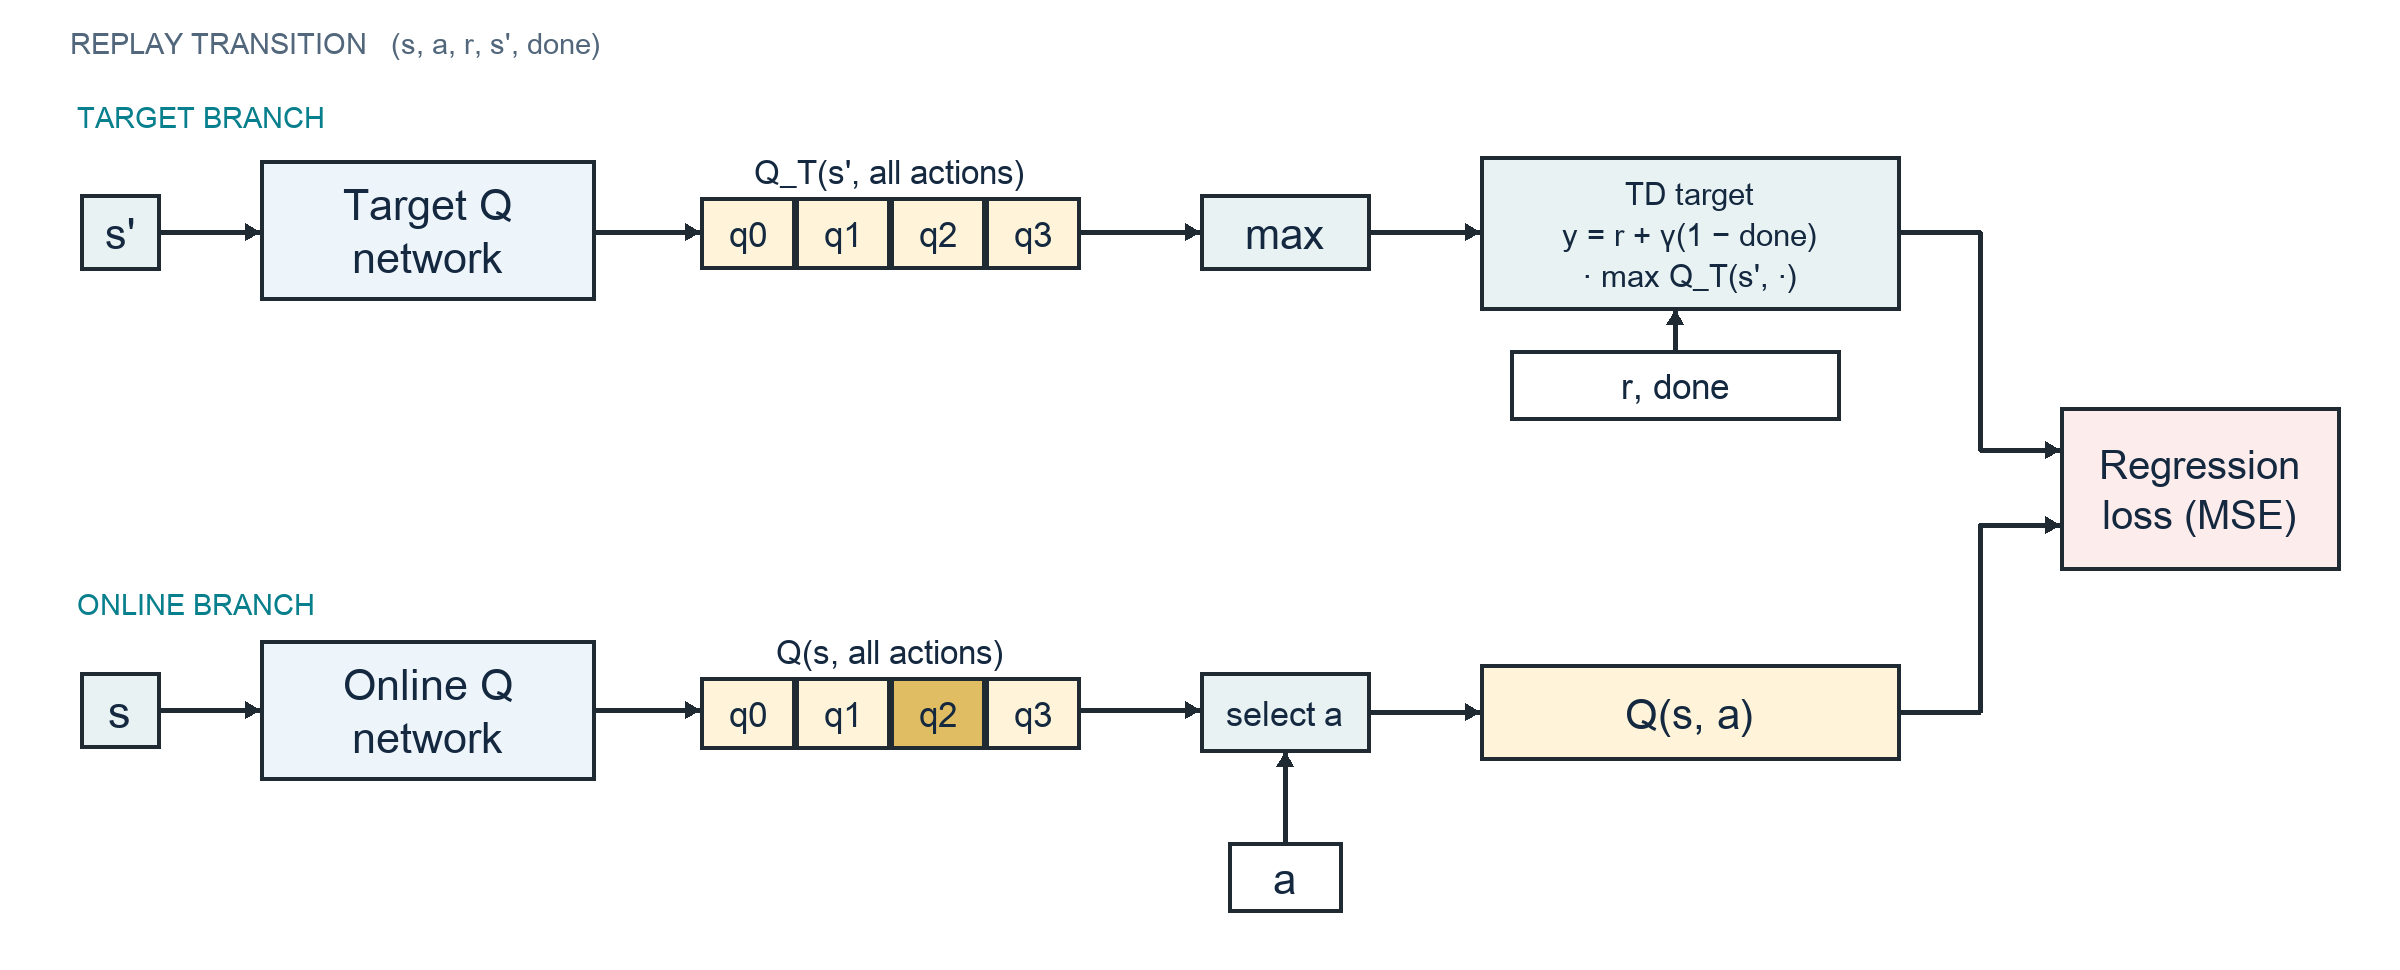
\includegraphics[width=\textwidth,height=5.55cm,keepaspectratio]{model-dqn.png}
\end{frame}

% 10 — ActorDQN architecture
\begin{frame}{Model Design: ActorDQN}
  \centering
  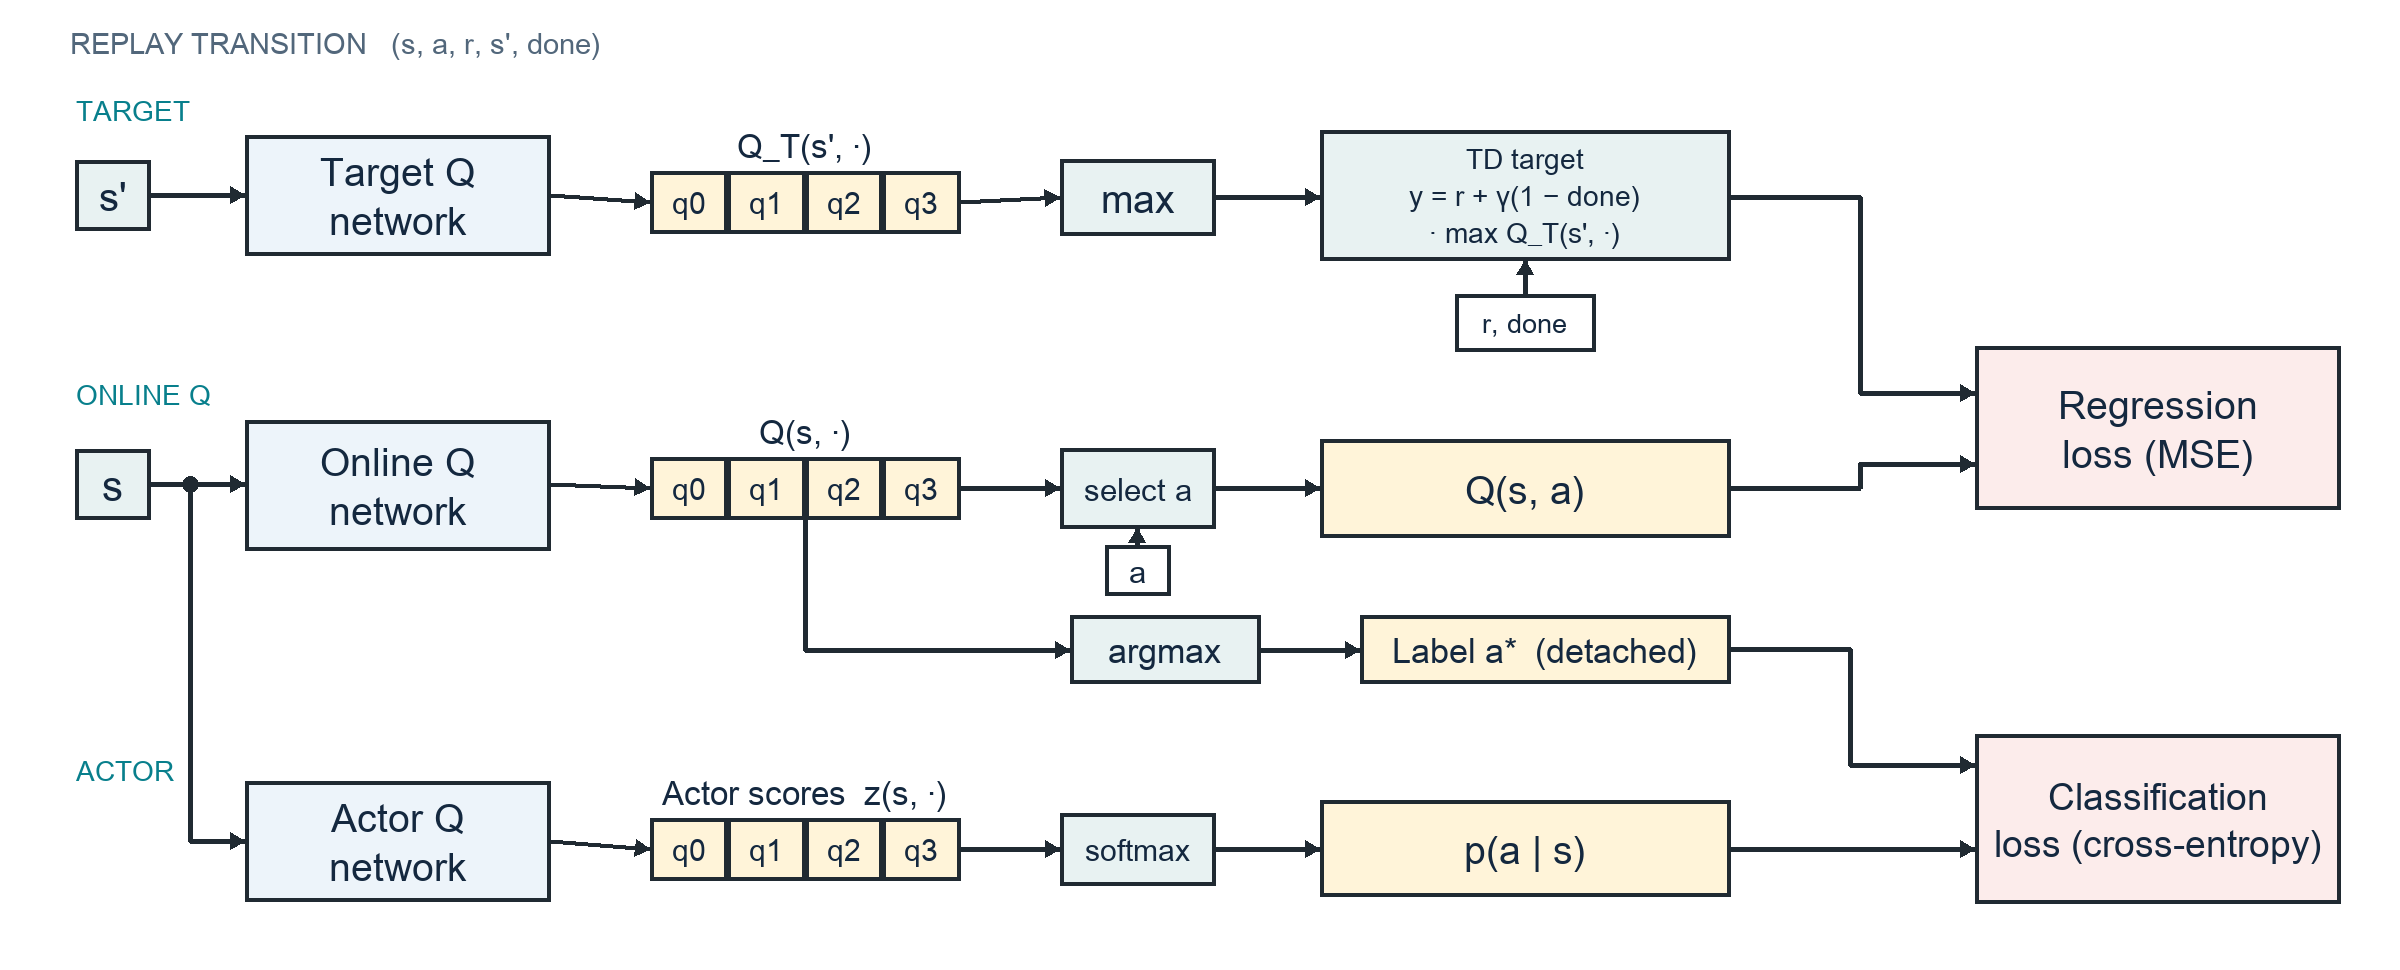
\includegraphics[width=\textwidth,height=5.55cm,keepaspectratio]{model-actordqn.png}
\end{frame}

% 11 — results outline
\begin{frame}{Experimental Results}
  \vspace{0.35cm}
  \begin{enumerate}\setlength{\itemsep}{0.70cm}
    \item \textbf{Performance in mazes}\par
      Full held-out sets for $4\times4$ and $5\times5$ mazes.
    \item \textbf{Justification for the idea}\par
  \end{enumerate}
\end{frame}

% 12 — 4x4 table
\begin{frame}{Performance in Maze: $4\times4$}
  \small Held-out set: 201 mazes per seed \quad Step limit: 160
  \vspace{0.55cm}
  \centering
  \renewcommand{\arraystretch}{1.70}
  \begin{tabular}{lcc}
    \toprule
    Policy & Success rate & Mean steps, successful mazes \\
    \midrule
    ActorDQN & $\mathbf{0.828\pm0.029}$ & $25.95\pm3.65$ \\
    Basic DQN & $0.111\pm0.072$ & $\mathbf{4.42\pm0.94}$ \\
    Uniform Random & $0.740\pm0.048$ & $63.86\pm4.04$ \\
    \bottomrule
  \end{tabular}
  \par\vspace{0.48cm}
  \small\color{muted}Mean $\pm$ sample SD across three seeds. 
\end{frame}

% 13 — 5x5 table
\begin{frame}{Performance in Maze: $5\times5$}
  \small Held-out set: 2,973 mazes per seed \quad Step limit: 250
  \vspace{0.55cm}
  \centering
  \renewcommand{\arraystretch}{1.70}
  \begin{tabular}{lcc}
    \toprule
    Policy & Success rate & Mean steps, successful mazes \\
    \midrule
    ActorDQN & $\mathbf{0.673\pm0.027}$ & $48.26\pm5.09$ \\
    Basic DQN & $0.129\pm0.036$ & $\mathbf{8.33\pm0.45}$ \\
    Uniform Random & $0.564\pm0.004$ & $122.25\pm1.22$ \\
    \bottomrule
  \end{tabular}
  \par\vspace{0.48cm}
  \small\color{muted}Mean $\pm$ sample SD across three seeds. 
\end{frame}

% 14 — gap table
\begin{frame}{Generalization Gap}
  \small Gap $=$ training-set mean $-$ held-out mean;
  \vspace{0.38cm}
  \centering
  \renewcommand{\arraystretch}{1.42}
  \setlength{\tabcolsep}{6pt}
  \begin{tabular}{llrrr}
    \toprule
    Maze & Policy & $\Delta$ steps, all
      & $\Delta$ steps, success & $\Delta$ success rate \\
    \midrule
    $4\times4$ & ActorDQN & $-6.07$ & $-2.92$ & $+0.026$ \\
                & Basic DQN & $-15.72$ & $+0.12$ & $+0.102$ \\
    \midrule
    $5\times5$ & ActorDQN & $-3.89$ & $-1.32$ & $+0.014$ \\
                & Basic DQN & $-1.83$ & $+0.03$ & $+0.008$ \\
    \bottomrule
  \end{tabular}
  \par\vspace{0.40cm}
  \small\color{muted}A smaller absolute gap is better.
\end{frame}

% 15 — probe architecture
\begin{frame}{Justification for the Idea}
  \small Two frozen teachers are tested separately: DQN target and ActorDQN target.
  \vspace{0.10cm}
  \centering
  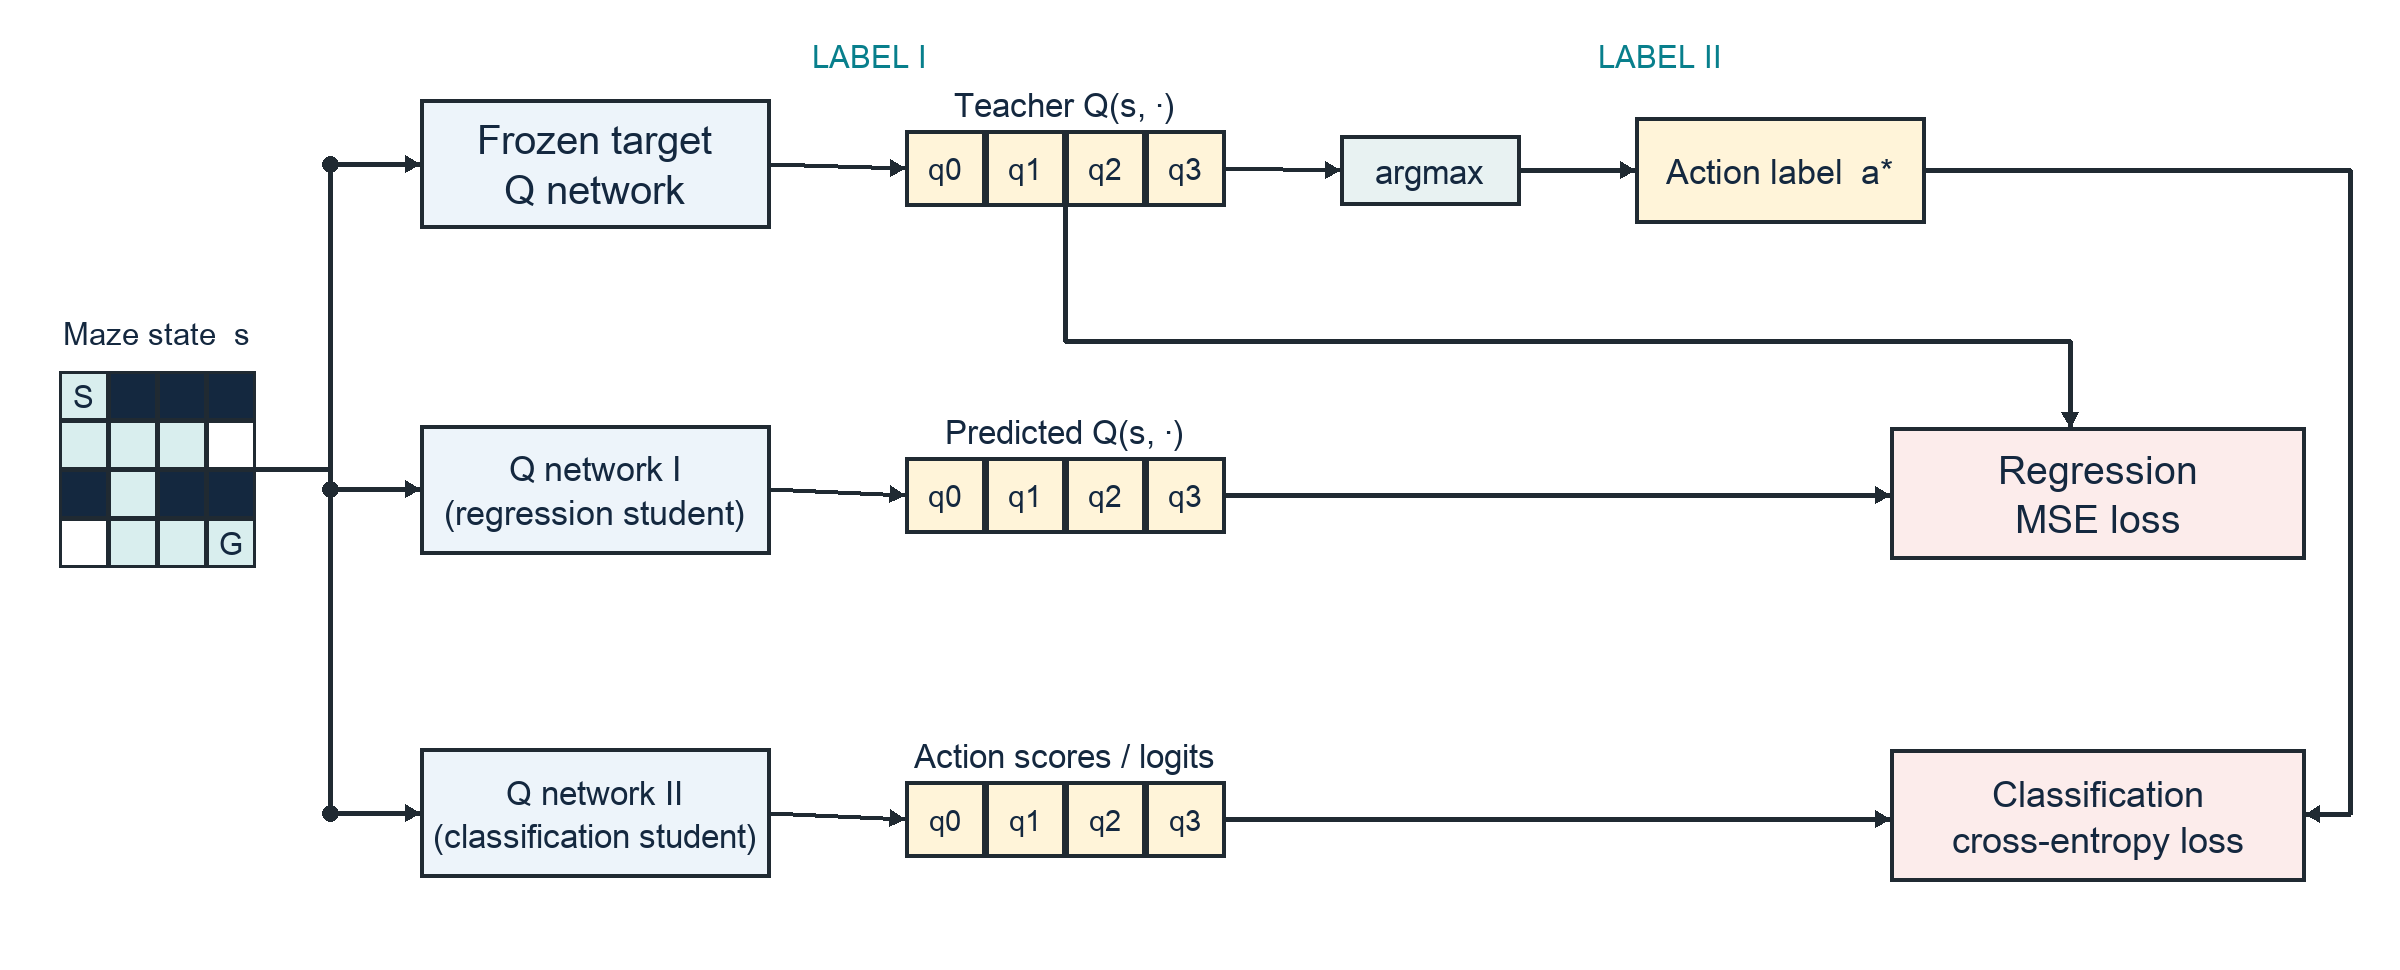
\includegraphics[width=\textwidth,height=5.10cm,keepaspectratio]{justification-flow.png}
  \par\vspace{0.10cm}
  \scriptsize\color{muted}Matched students share architecture, initialization, minibatches, and update budget.
\end{frame}

% 16 — probe table
\begin{frame}{Classification vs. Q-value Regression}
  \centering
  \renewcommand{\arraystretch}{1.42}
  \setlength{\tabcolsep}{4.5pt}
  \begin{tabular}{llccc}
    \toprule
    Teacher & Objective
      & \shortstack{Agreement\\10k updates}
      & \shortstack{Agreement\\102.4k updates}
      & \shortstack{Maze success\\102.4k updates} \\
    \midrule
    DQN & Classification & $\mathbf{0.868}$ & $\mathbf{0.899}$ & $\mathbf{137/201\;(0.682)}$ \\
        & Regression & $0.800$ & $0.853$ & $116/201\;(0.577)$ \\
    \midrule
    ActorDQN & Classification & $\mathbf{0.964}$ & $\mathbf{0.967}$ & $\mathbf{175/201\;(0.871)}$ \\
             & Regression & $0.910$ & $0.955$ & $162/201\;(0.806)$ \\
    \bottomrule
  \end{tabular}
  \par\vspace{0.35cm}
  \small\color{muted}Action agreement means matching the teacher's greedy action on held-out observations.
\end{frame}

\end{document}
